\chapter{Osciladores LC}
\label{osciladores-lc}
\chapterprecis{Em aplicações RF é mais comum empregar redes de realimentações utilizando somente tanques LC, devido ao alto fator de qualidade, podendo, também, assumir potências extremamentes altas (ao contrário, por exemplo, de redes com amplificadores operacionais). Alguns desses osciladores são: oscilador LC MOS, royer e mazzilli.}\index{sinopse de capítulo}
\section{Oscilador LC MOS cruzado acoplado}
Neste tipo de oscilador, os transistores estão em classe A (ver \autoref{fig_lc-mos}), fornecendo energia ao tanque LC, consumida devido às perdas dos componentes. Neste caso, a energia que o transistor injeta no tanque, deve ser maior ou igual que a resistência de perda total do circuito. O fator de qualidade deste circuito é:
\begin{equation}
Q = \frac{2\pi f L}{R_p}
\end{equation}
E o $g_m$ é:
\begin{equation}
g_m = \frac{i_D}{V_{GS} - V_t}
\end{equation}
Para que ocorra uma oscilação:
\begin{equation}
\frac{1}{g_m} \geq \frac{2\pi f L}{Q}
\end{equation}
É importante notar que, mesmo que o circuito seja instável e os transistores entrem em corte e saturação, a tensão na saída continuará próxima de uma senoide para fatores de qualidade do tanque elevados.
Uma das grandes desvantagens desse circuito deve-se ao fato de que são poucos os MOSFETs que sustentam uma tensão de gate maior que 20V, limitando assim a potência do circuito.

\begin{figure}[htb]
\caption{\label{fig_lc-mos}O oscilador LC MOS}
\begin{center}
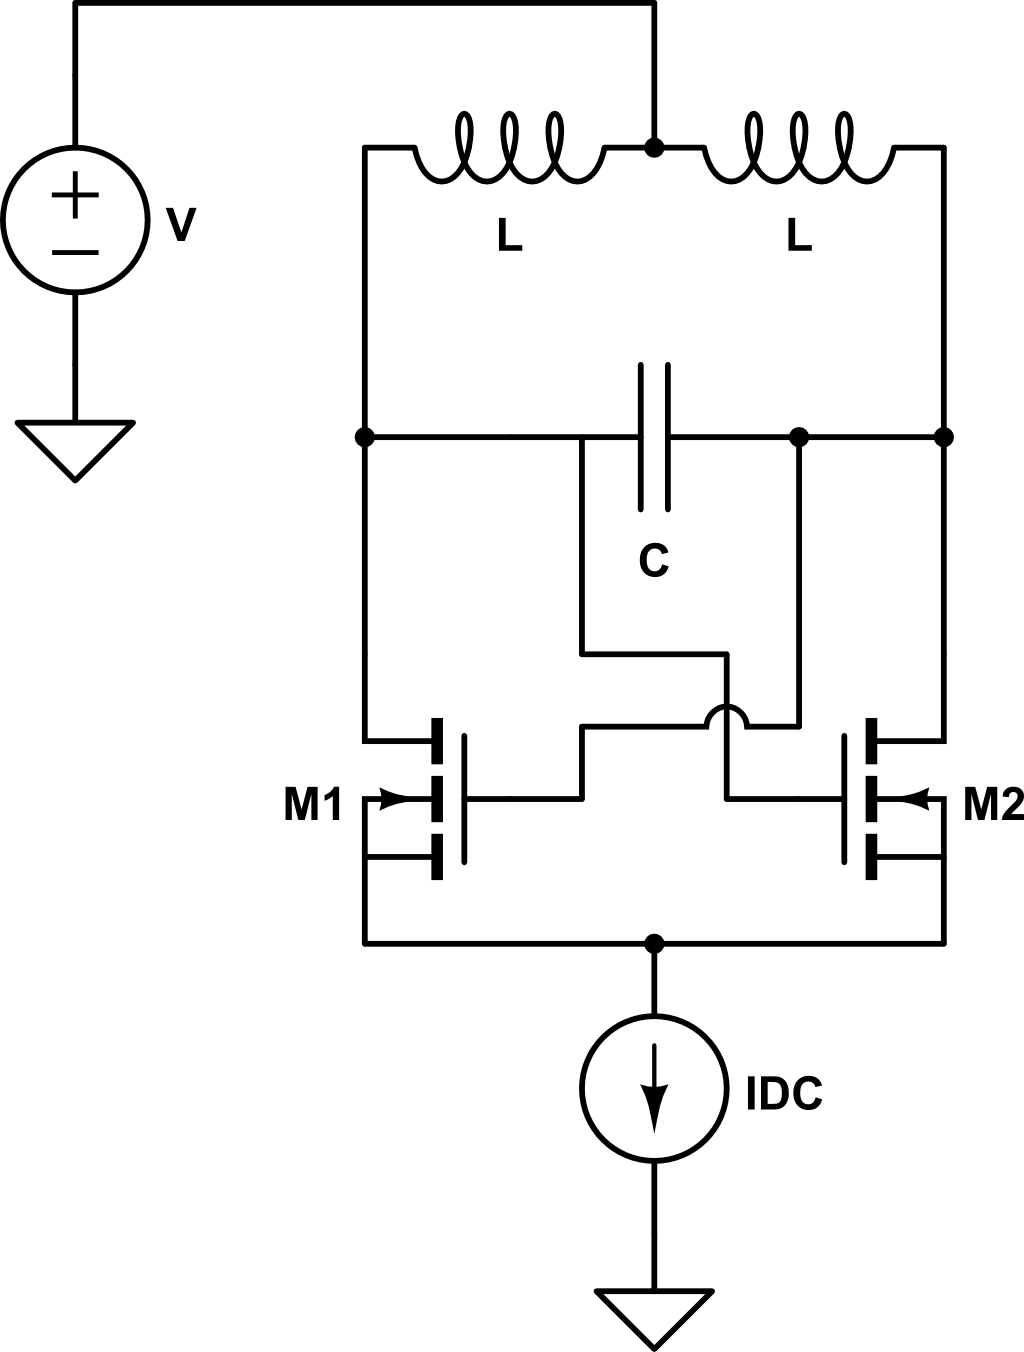
\includegraphics[scale=0.5]{images/lc-mos.png}
\end{center}
\end{figure}

\section{Oscilador Royer}
Em 1954, George Royer patenteou o oscilador Royer (\autoref{fig_royer}), um circuito auto ressonante, simples e com pouco uso de componentes. Como a maioria dos osciladores, ele utiliza um tanque LC para a oscilação. A grande vantagem deste circuito consiste no uso de um terceiro enrolamento conectado à base dos transistores, isto garante que um transistor estará cortado enquanto o outro estiver conduzindo, diminuindo drasticamente o consumo de energia do circuito.

\begin{figure}[htb]
\caption{\label{fig_royer}Oscilador Royer}
\begin{center}
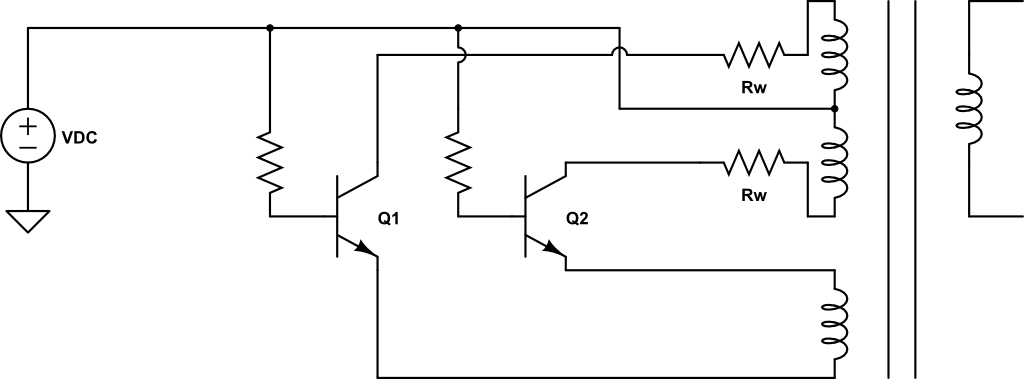
\includegraphics[scale=0.5]{images/royer-oscillator.png}
\end{center}
\end{figure}

\section{Oscilador Mazzilli}
O oscilador Mazzilli\cite{paolucci2009novel}\cite{mcclusky2010high}, mostrado na \autoref{fig_mazzilli}, é uma derivação do oscilador Royer com o LC MOS. A grande diferença consiste no circuito presente no gate, para assegurar o baixo consumo energético e o chaveamento em ZVS\footnote{\emph{Zero-Voltage Switching} ocorre que o MOSFET só irá alternar de um estado para o outro quando a tensão do dreno for zero, reduzindo a perda, que normalmente é transformado em calor, do circuito}(\autoref{fig_zvs}) sem o uso de um terceiro enrolamento no indutor. O oscilador Mazzilli retira energia de Vin (como no Royer) e, no entanto, liga os gates, por meio de diodos, ao dreno oposto. Com isso, suprimos o problema de tensão que existia no LC MOS e continuamos a utilizar MOSFET ao invés de BJT, podendo assim, garantir alta frequência de oscilação.

\begin{figure}[h]
\caption{\label{fig_zvs}Simulação realizada no Orcad que mostra o chaveamento em ZVS}
\begin{center}
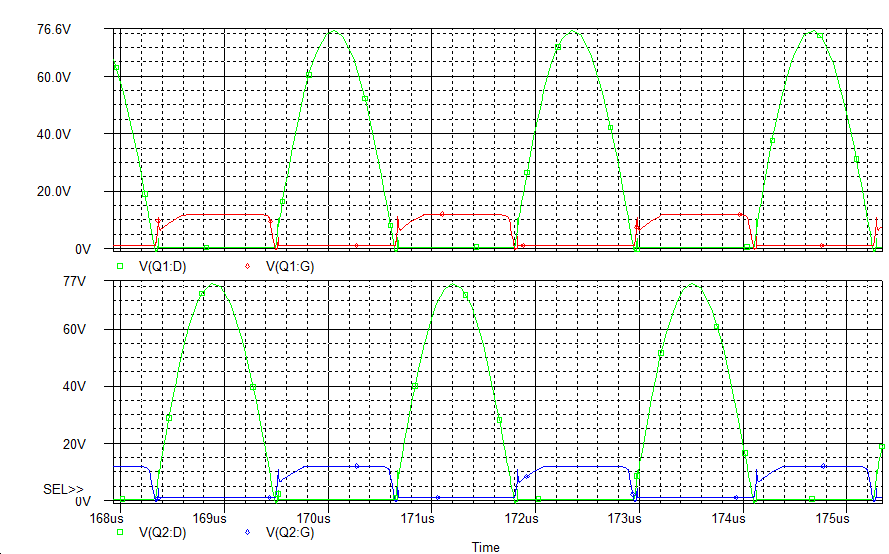
\includegraphics[scale=0.5]{images/zvs.png}
\end{center}
\legend{Observa-se que a troca de um modo de operação para outro no FET ocorre somente quando há uma tensão zero, diminuindo assim o gasto energético, e, consequentemente, a dissipação de calor.}
\end{figure}

\begin{figure}[h]
\caption{\label{fig_mazzilli}Oscilador Mazzilli}
\begin{center}
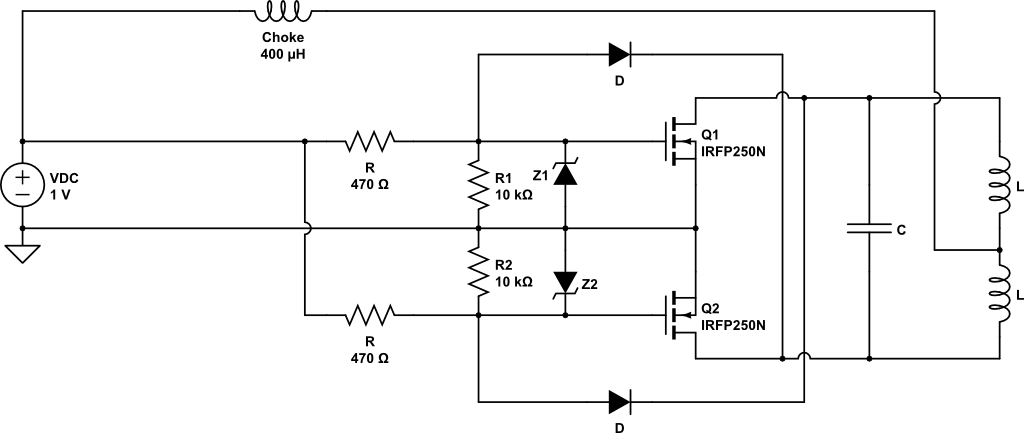
\includegraphics[scale=0.5]{images/mazzilli.png}
\end{center}
\legend{Observe a semelhança com o oscilador LC MOS}
\end{figure}

\subsection{Modos de Operação}
%Esse conversor possui quatro modos de operação. O primeiro modo o dreno das duas chaves estão aterrados. Como a ligação é cruzada, garantimos que a chave 1 está cortada e a 2 ativa. Durante esta operação o capacitor é completamente descarregado. Depois disso a chave 1 é cortada e é a vez da chave 2 está ativa. Assim há a geração de uma corrente que irá percorrer o tanque LC e irá descarregar na chave ativa. Quando a voltagem no dreno 1 retorna para zero, ocorre o chaveamento das duas chaves. Assim como no modo de operação 1 o capacitor está completamente descarregado, e o indutor carrega totalmente a corrente em posição oposta. E finalmente, o modo 4 que ocorre exatamente o mesmo evento que o modo 2, no entanto, na chave 1.

Com a chave 1 indo para o modo ativa e a chave 2 indo para corte temos o primeiro modo de operação (\autoref{fig_mazzilli-1}). O dreno da chave 1 provê um aterramento para a corrente DC do circuito. Ambos os drenos estão com tensão zero, curto circuitando o capacitor. Toda energia do tanque está neste momento armazenada na corrente de pico do indutor. Como o circuito opera com ZVS, nenhuma corrente AC do tanque passa pelas chaves. 

\begin{figure}[htb]
\caption{\label{fig_mazzilli-1}Modo 1 de operação do Oscilador Mazzilli}
\begin{center}
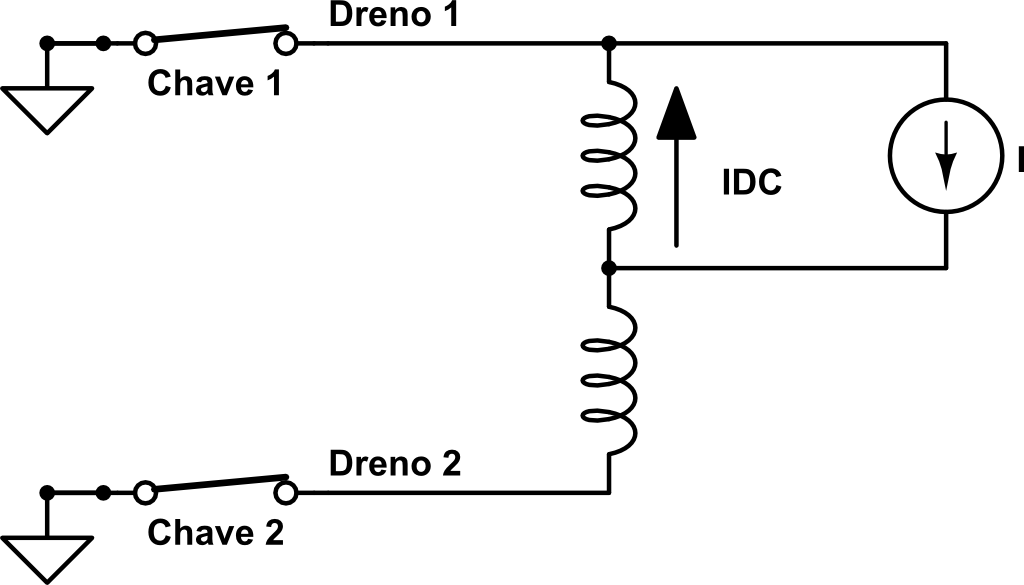
\includegraphics[scale=0.3]{images/mazzilli-1.png}
\end{center}
\legend{Momento em que os transistores estão chaveando para os seus modos. A chave 1 indo para o modo ativo e a chave 2 para o corte.}
\end{figure}

Com a chave 2 em corte, o segundo modo de operação pode ser visto como a elevação e a queda da tensão do capacitor (\autoref{fig_mazzilli-2}). A corrente no indutor carrega o capacitor até a tensão máxima de dreno até a metade de tempo do segundo modo de operação do circuito. Com o pico da tensão de dreno em 2, toda a energia do ressonador é armazenado no capacitor. Após isto, o capacitor começa a se descarregar, transferindo a energia de volta para os indutores. 

\begin{figure}[h!tb]
\caption{\label{fig_mazzilli-2}Modo 2 de operação do Oscilador Mazzilli}
\begin{center}
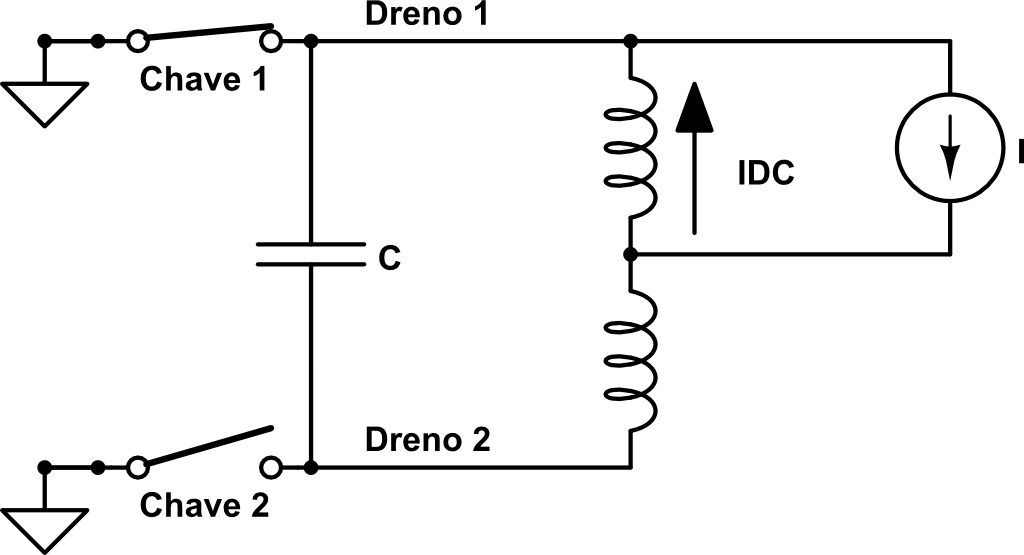
\includegraphics[scale=0.3]{images/mazzilli-2.png}
\end{center}
\end{figure}

O modo 3 mostrado na \autoref{fig_mazzilli-3}, ocorre quando a tensão do nó 2 atinge zero. O MOSFET em push-pull é então chaveado, fornecendo um caminho para a corrente DC até o terra pela chave 2. Por fim, o último modo de operação ocorre de forma similar que o modo 2, no entando com a chave 2, como pode ser visto na \autoref{fig_mazzilli-4}.

\begin{figure}[h!tb]
\caption{\label{fig_mazzilli-3}Modo 3 de operação do Oscilador Mazzilli}
\begin{center}
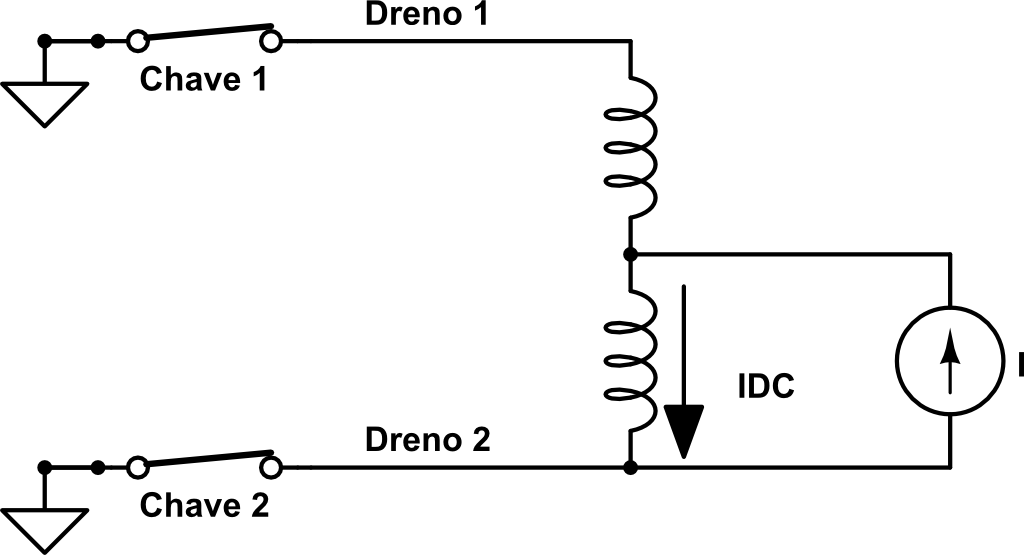
\includegraphics[scale=0.3]{images/mazzilli-3.png}
\end{center}
\legend{Momento em que os transistores estão chaveando para os seus modos. A chave 1 indo para o corte e a chave 2 para o modo ativo.}
\end{figure}

\begin{figure}[htb]
\caption{\label{fig_mazzilli-4}Modo 4 de operação do Oscilador Mazzilli}
\begin{center}
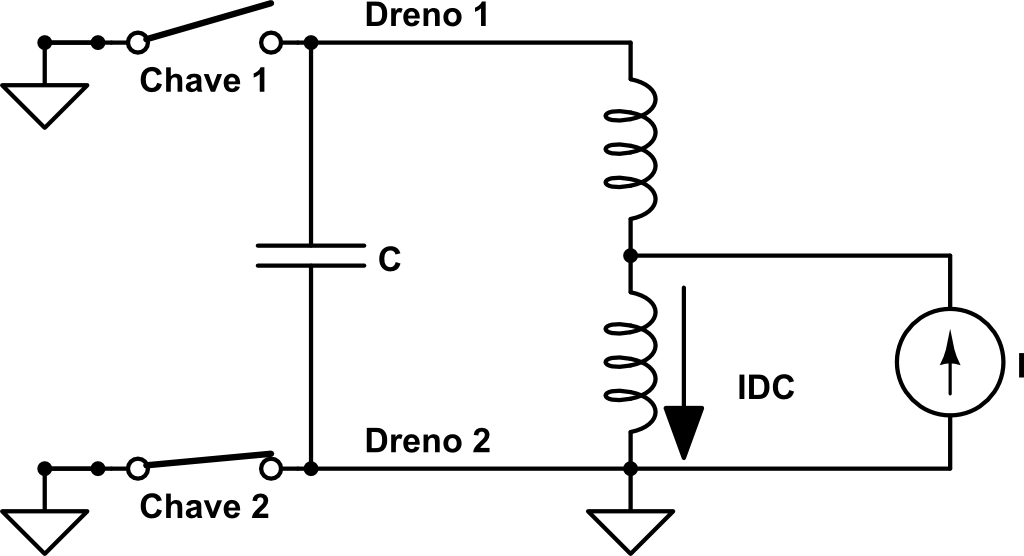
\includegraphics[scale=0.3]{images/mazzilli-4.png}
\end{center}
\end{figure}

\subsection{Limitações do circuito}

\subsubsection{Dependência da carga}
Durante a transferência de potência a carga é refletida para o primário, e aparece em paralelo com o tanque LC, e com isso a frequência de oscilação é dependente da carga em uso, gerando uma perda maior.
\subsubsection{Resposta do Gate}
Quando a frequência de oscilação é baixa, este fator não é crucial. No entanto, com o aumento de frequência, o tempo de resposta do transistor pode interferir no funcionamento do circuito.

\subsubsection{Alta voltagem no Gate}
Outro problema é a alta voltagem presente no gate. Este problema é facilmente mitigado adicionando um zener com uma tensão ligeiramente abaixo da tensão de breakdown do gate (\autoref{fig_gate}), embora cause uma perda maior na resistência do gate.

\begin{figure}[htb]
\caption{\label{fig_gate}Oscilador Mazzilli}
\begin{center}
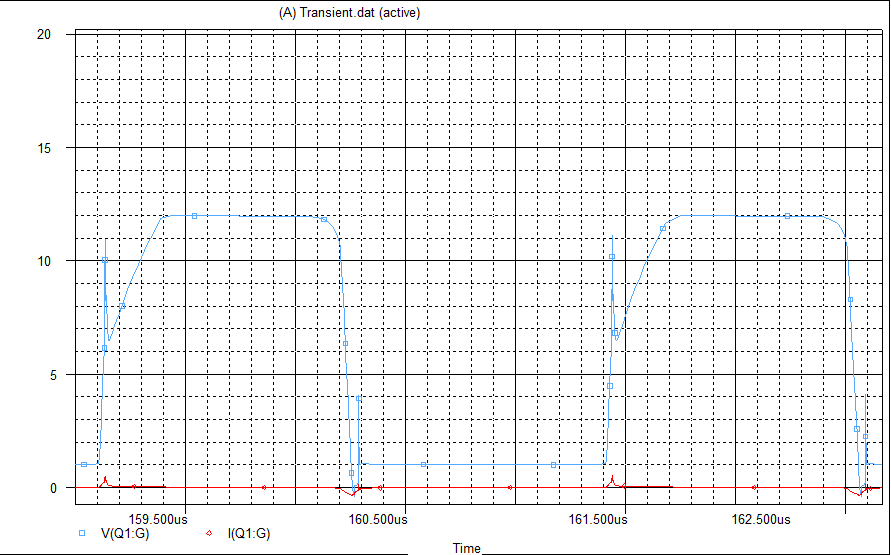
\includegraphics[scale=0.5]{images/gate.png}
\end{center}
\legend{A tensão no gate é limitada pelo Zener de 12V na simulação realizada no Orcad}
\end{figure}

\subsection{Resistência do transistor}
Quando o transistor está descarregando o capacitor, toda a corrente gerada no circuito passa através dele. Por isso, há a necessidade de optar por um MOSFET que possua a menor resistência possível quando ele estiver conduzindo, afim de manter a menor perda possível no transistor de forma a mitigar a dissipação de calor.